\centering{\textbf{ก่อนศึกษารายละเอียดเกี่ยวกับการเคลื่อนที่แบบวงกลม นักเรียนต้องทำความเข้าใจคำศัพท์ต่อไปนี้ให้ดีก่อน}}
\tcblower
\begin{minipage}{.6\textwidth}
	\begin{itemize}[leftmargin=*]
		\item[1)] คาบ (T)  คือเวลาที่ใช้ในการเคลื่อนที่ครบ  1 รอบ มีหน่วยเป็นวินาที (s)
		\item[2)] ความถี่ (f)  คือจำนวนรอบที่เคลื่อนที่ได้ในหนึ่งหน่วยเวลามีหน่วยเป็น  รอบ/วินาที  หรือเฮิรตซ์ (Hz)  เราสามารถหาค่าความถี่ได้จากสมการต่อไปนี้ \\
				  $$f = \frac{\text{จำนวนรอบ}}{\text{เวลา}} \quad \text{หรือ} \quad f = \frac{1}{T}$$
				\begin{tabbing}
					\textbf{เมื่อ} \quad 	\=f \quad\=\textbf{คือ}ความถี่ (Hz) \\
										\>T \>\textbf{คือ}คาบของการเคลื่อนที่ (วินาที)
				\end{tabbing}
	\end{itemize}
\end{minipage}
\hfill
\begin{adjustbox}{valign=c} 
    \begin{minipage}[t]{.35\linewidth}
        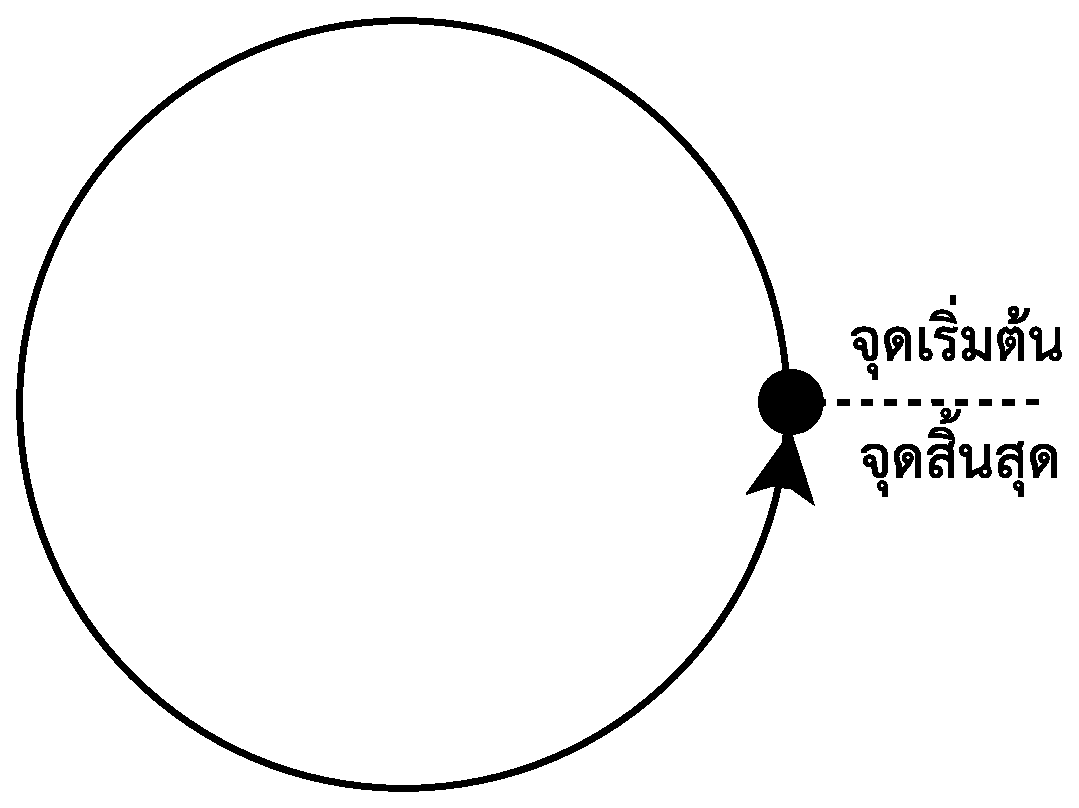
\includegraphics[width=\linewidth]{content-11.eps}
    \end{minipage}
\end{adjustbox}
